\chapter{Theoretische Grundlagen}
\label{cha:Grundlagen}
In diesem Kapitel werden Theoretische Grundlagen geschaffen, die zum weiteren Verständnis der Arbeit benötigt werden. Zuerst werden ausgewählte Video-Schnittstellen erläutert und verglichen und bewertet welchen praktischen Nutzen diese für handelsübliche embedded Linuxsysteme bietet. Im Weiteren werden zwei Linux Boards verglichen und bewertet sowie deren praktische Einsatzgebiete beispielhaft dargelegt.

\section{Video-Schnittstellen}
Unter Video-Schnittstellen kann man die Schnittstellen verstehen, die direkt zur Anzeige von Bilddaten dienen und physikalisch mit einer Anzeigeeinheit verbunden sind. Hier können sowohl Hardware- als auch Softwarekomponenten enthalten sein.
\subsection{VGA}
Unter VGA versteht man Video Graphics Array und wurde 1987 von IBM entwickelt. Der Stecker hat 15 Pins und liefert neben analogen Farbinformationen Horizontale und Vertikale Synchronisationssignale. Aufgrund der limitierten Spezifikationen ist die Schnittstelle eher antik und selbst Intel als Chiphersteller will ab 2015 auf die Schnittstelle verzichten \cite{Intel2010} und digitalen Schnittstellen den Vorzug lassen. Zwar ist die VGA-Schnittstelle noch nicht komplett wegrationalisiert, so wird sie den digitalen Schnittstellen trotzdem weichen müssen. Der Trend bei embedded Linuxsystemen ist zumindest der, dass handelsübliche Systeme direkt mit HDMI oder anderen digitalen Schnittstellen entwickelt werden.

\subsection{DVI}
Hinter DVI steht der Begriff Digital Visual Interface und stellt ein digitale Schnittstelle zur Grafikanzeige dar. Der DVI Standard wurde 1999 von der DDWG\footnote{Digital Display Working Group} verabschiedet, da der Wunsch nach Leistungsstärkeren Schnittstellen vorhanden war. QXGA-Auflösungen\footnote{QXGA: 2048x1536} sind auf analogem Wege nicht mehr befriedigend erzielbar. Die DVI Schnittstelle beinhaltet neben den Digitalen Signalen zusaetzlich analoge VGA Signale, was den Betrieb älterer Monitore und Displays zulässt. Zur digitalen Datenübertragung wird der TMDS\footnote{Transition Minimized Differential Signaling - Differentielle Datenübertragung} Standard verwendet, welcher die 24 Bit Farbinformationen\footnote{24 Bit: je 8 Bit für Rot, Grün und Blau} mittels eines Serializers in serielle Daten umwandelt. Je nach benötigter Bandbreite können drei oder sechs Aderpaare für Pixeldaten verwendet werden. Dies wird Single-Link bzw. Double-Link genannt und es lassen sich dabei max. 3.72 GBit/s\footnote{max. UXGA: 1600x1200@60Hz} bzw. 7.44 GBit/s\footnote{max. WUXGA: 1920x1200@60Hz} übertragen. Um die Paare zuordnen zu können, wird ein weiteres Paar zur Synchronisation verwendet. Um die Uebertragung noch effizienter zu gestalten, gibt es die Moeglichkeit bei High- sowie Low-Pegel des Taktsignals Daten zu übertragen\footnote{Double Data Rate} \cite{Leunig2002}.

\begin{figure}[hb]
	\centering
	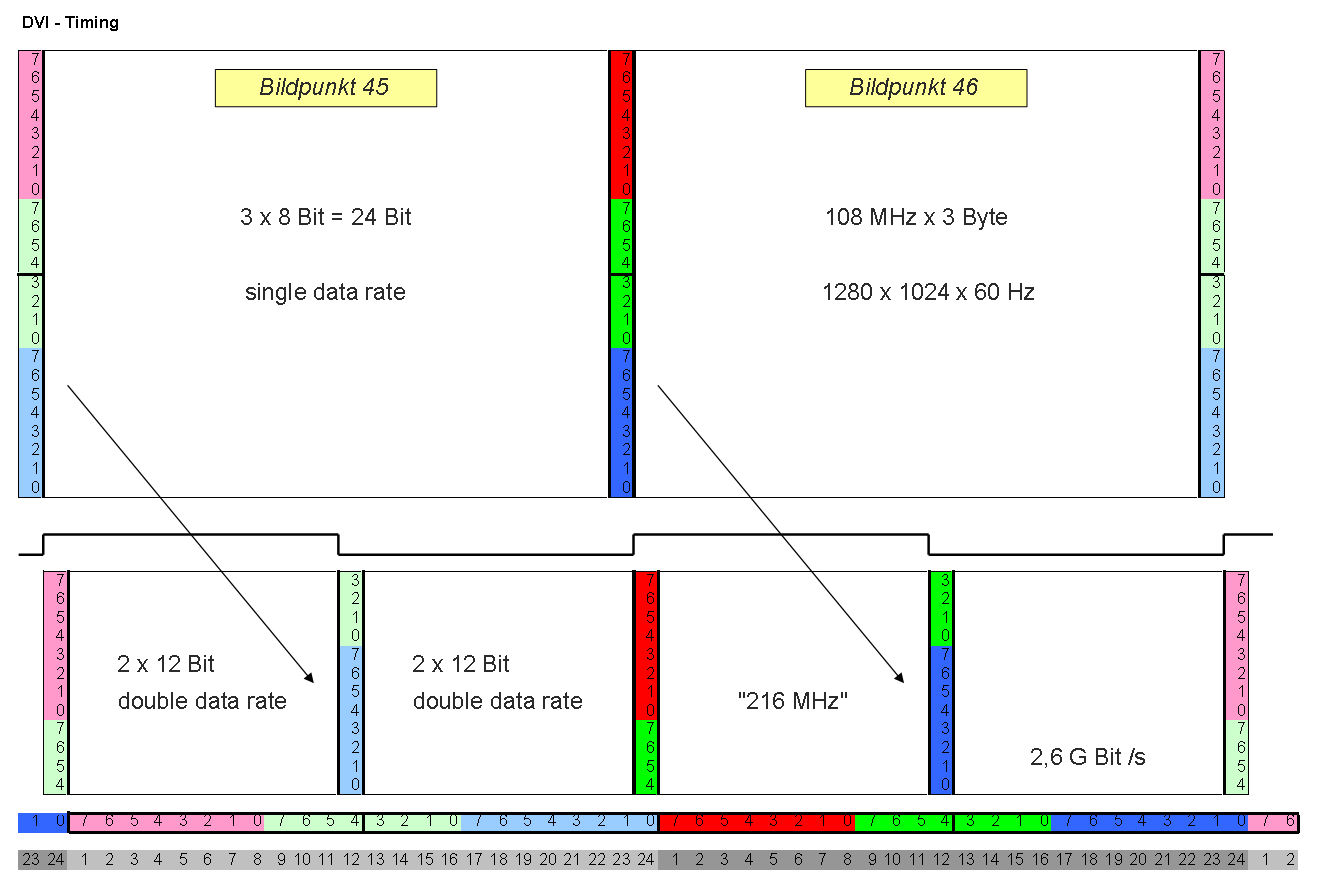
\includegraphics[width=textwidth]{Grundlagen/dvi_timing.png}
	\caption{Quelle: DVI-Timing, \cite{Wikipedia2010a}}
	\label{fig:dvi_timing}
\end{figure}
\label{fig:dvi_timing} zeigt ein Timing Diagramm, welches die Datenübertragung darstellt. Der Obere Teil des Bildes zeigt die Übertragung bei nicht aktiver, unten bei aktiver Double Data Rate. Die Taktleitung in der Mitte wird bei aktiver Double Data Rate voll ausgenutzt. \\

Fuer 

\subsection{HDMI}

\subsection{TV-OUT}
\subsection{LVDS}
\subsection{8080-Interface}
\subsection{Verwendung der SPI-Schnittstelle}
\subsection{Bewertung der Video-Schnittstellen}

\section{Betrachtete Embedded Linux Boards}
\subsection{Raspberry Pi}
\subsection{Gnublin Extended}
\subsection{Bewertung der Linux-Boards}
